\documentclass[border=3pt,tikz]{standalone}
\usepackage{tikz}
\usepackage{amsmath} % for \text
\usepackage{mathrsfs} % for \mathscr -> scri
\usepackage{xfp} % for fpeval -> floating point expression

\newcommand{\scri}{\mathscr{I}} %\mathcal
\tikzset{>=latex} % for LaTeX arrow head
\newcommand\height[1]{ sqrt(1/(1+#1)+#1^2) }
\newcommand\samp[1]{ tan(90*#1) }
\tikzset{declare function={%
  paramT(\r,\t)  = {\fpeval{1/pi*(atan(\t+\height{\r}+\r) + atan(\t+\height{\r}-\r))}};
  paramR(\r,\t)  = {\fpeval{1/pi*(atan(\t+\height{\r}+\r) - atan(\t+\height{\r}-\r))}};
}}

\begin{document}

% PENROSE DIAGRAM of Minkowski space
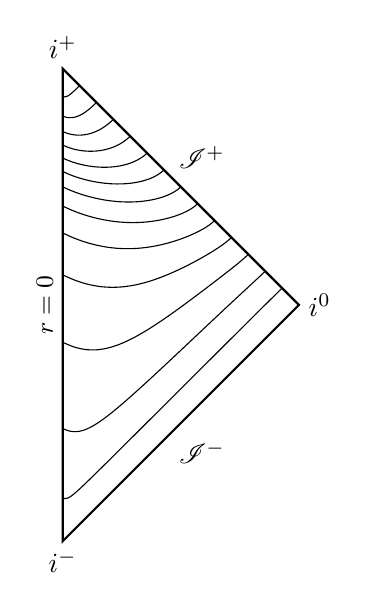
\begin{tikzpicture}[scale=3]
    \def\Nlines{6} % number of lines for t>0
    \coordinate (O) at ( 0, 0); % center: origin (r,t) = (0,0)
    \coordinate (S) at ( 0,-1); % south: t=-infty, i-
    \coordinate (N) at ( 0, 1); % north: t=+infty, i+
    \coordinate (E) at ( 1, 0); % east:  r=+infty, i0

    % LABELS
    \node[right] at (E) {$i^0$};
    \node[above] at (N) {$i^+$};
    \node[below] at (S) {$i^-$};
    \node[above, rotate=90] at (O) {\small{$r=0$}};
    \node[above right] at (50:0.7) {$\scri^+$};
    \node[below right] at (-50:0.7) {$\scri^-$};
    
    % FOLIATION
    \message{Making world lines...^^J}
    \foreach \i [evaluate={\c=\i/(\Nlines+1);}] in {-\Nlines,...,\Nlines}{
      \message{  Running i/N=\i/\Nlines, c=\c...^^J}
      \draw[line width=0.4,samples=20,smooth,variable=\r,domain=0.001:1]
        plot({ paramR(\samp{\r},\samp{\c}) }, { paramT(\samp{\r},\samp{\c}) });    % c>0
    }
    
    \draw[thick] (N) -- (E) -- (S) -- cycle;
    
%    % T-ARROW 
%    \draw[->,shorten <=0.4]
%      ( { paramR(\samp{0.6},\samp{(\Nlines-6)/(\Nlines+1)}) }, { paramT(\samp{0.6},\samp{(\Nlines-6)/(\Nlines+1)}) } )
%      to[out=60,in=180]++ (25:0.25)
%      node[right=-2] {\small{$t=\text{const}$}};          

  \end{tikzpicture}
\end{document}